\documentclass{article}
\usepackage[italian]{babel}
\usepackage[tmargin=2cm,rmargin=1.5in,lmargin=1.5in,margin=0.85in,bmargin=2cm,footskip=.2in]{geometry}
\usepackage{siunitx}
\sisetup{separate-uncertainty=true, per-mode=fraction, parse-numbers=true}
\usepackage{caption}
\usepackage[T1]{fontenc}
\usepackage{bookmark}
\usepackage{mathcomp}
\usepackage{graphicx}
\usepackage{multicol}
\usepackage{booktabs}
\usepackage{amsmath,amsfonts,amsthm,amssymb,mathtools}
\hypersetup{
	pdftitle={Relazione sul pendolo quadrifilare},
	colorlinks=true, linkcolor=doc!90,
	bookmarksnumbered=true,
	bookmarksopen=true
}
\usepackage{blindtext}
\usepackage{wrapfig}
\usepackage{listings}
\usepackage{xcolor}
\usepackage{float}
\usepackage{tikz}
\usepackage{multirow}
\usepackage{biblatex}
\definecolor{codegreen}{rgb}{0,0.6,0}
\definecolor{codegray}{rgb}{0.5,0.5,0.5}
\definecolor{codepurple}{rgb}{0.58,0,0.82}
\definecolor{backcolour}{rgb}{0.95,0.95,0.92}
\definecolor{doc}{rgb}{0,0,0}
\lstdefinestyle{code}{
    backgroundcolor=\color{backcolour},   
    commentstyle=\color{codegreen},
    keywordstyle=\color{magenta},
    numberstyle=\tiny\color{codegray},
    stringstyle=\color{codepurple},
    basicstyle=\ttfamily\footnotesize,
    breakatwhitespace=false,         
    breaklines=true,                 
    captionpos=b,                    
    keepspaces=true,                                     
    showspaces=false,                
    showstringspaces=false,
    showtabs=false,                  
    tabsize=2,
    inputencoding=ansinew,
    extendedchars=true,
    numbers=left,                    
    numbersep=5pt
}

\lstset{style=code}
\usepackage[varbb]{newpxmath}
\usepackage{circuitikz}
\captionsetup{labelfont={bf, sc}}
\title{Relazione sul pendolo quadrifilare}
\author{Francesco Sermi}
\date{\today}
\begin{document}
	\maketitle
	\newpage
	\tableofcontents
	\newpage
	\section{Scopo}
		Stabilire la dipendenza che sussiste fra il periodo dell'oscillazione e la sua ampiezza
	\section{Cenni teorici}
	Il pendolo fisico (o il pendolo semplice, che può essere visto come caso particolare del pendolo fisico) può essere schematizzato come un corpo rigido soggetto ad una forza peso che induce un momento torcente rispetto al perno $O$ e la reazione vincolare $R$ che agiscono sulla massa $m$, da cui si ricava utilizzando la $II^a$ cardinale:
	\begin{equation}
		\frac{d\vec{L}}{dt} = I\ddot{\theta} = -mgl\sin{\theta}
	\end{equation}
	che è un problema di Cauchy ben definito
	\begin{align}
		\begin{cases*}
			\ddot{\theta} = - \frac{mgL}{I} \sin{\theta} \\
			\theta(0) = \theta_0 \\
			\dot{\theta}(0) = 0
		\end{cases*}
	\end{align}
	da cui, utilizzando l'ipotesi delle piccole oscillazioni e considerando l'espansione in serie di Taylor della funzione $\sin{(x)} = \sum\limits_{n=0}^{+\infty} \frac{(-1)^n}{(2n+1)!} x^{2n+1}$, possiamo ricondurlo all'equazione di un oscillatore armonico:
	\begin{equation*}
		I\ddot{\theta} = -mgl\theta \implies \ddot\theta = -\frac{mgL}{I}\theta
	\end{equation*}
	Da cui si ricava che, ponendo $-\omega^2 = -\frac{mgL}{I}$, che il periodo di oscillazione è pari a
	\begin{equation*}
		T = 2\pi \sqrt{\frac{I}{mgL}}
	\end{equation*}
	da cui si vede che il periodo di oscillazione non dipende, nell'ipotesi delle piccole oscillazioni, dall'angolo di oscillazione iniziale $\theta_0$. \\	
	Se non ipotizziamo le piccole oscillazioni, si può dimostrare che, partendo dal problema di Cauchy di prima
	\begin{align*}
		\ddot{\theta} \cdot 2 \dot{\theta} = -2\frac{mgL}{I}\dot{\theta}\sin{\theta} \implies \int_0^T \frac{d\dot{\theta}^2}{dt} dt = \int_0^T -2\frac{mgL}{I}\dot{\theta}\sin{\theta} dt \implies \dot{\theta}^2 = \frac{2mgL}{I}(\cos{\theta} - \cos{\theta_0})
	\end{align*}
	da cui possiamo 
	\begin{align*}
		&\dot{\theta} = \pm \sqrt{\frac{2mgL}{I}(\cos{\theta} - \cos{\theta_0})} \implies \pm \frac{d\theta}{\sqrt{\frac{2mgL}{I}(\cos{\theta} - \cos{\theta_0})} } = dt
	\end{align*}
	e, integrando e sfruttando l'espansione in serie del coseno, è possibile dimostrare che
	\begin{equation*}
		T = T_0 \left( 1 + \frac{1}{16}\theta_0^2 + \frac{11}{3072}\theta_0^4 + \cdots \right)
	\end{equation*}
	dove $T_0 = 2\pi\sqrt{\frac{l}{g}}$
	Ragionando in termini energetici, si osserva che l'energia meccanica si conserva nel moto (supponendo che non ci siano attriti) del pendolo e si ha che
\begin{table}[htbp]
    \centering
    \begin{tabular}{l c}
        $E_0 = mg(l-l\cos{\theta})$ & \multirow{2}{*}{$\implies \theta_0 = \arccos{ \left(1 - \frac{v_0^2}{2gL} \right)}$} \\
         $E_0 = \frac{1}{2}mv_0^2$ &  \\
    \end{tabular}
\end{table}
	\section{Strumenti e materiali}
	\textbf{Materiali}:
	\begin{itemize}
		\item Pendolo quadrifilare;
	\end{itemize}
	\textbf{Strumenti}:
	\begin{itemize}
		\item Computer con programma di acquisizione;
		\item Metro a nastro, con sensibilità pari a $\pm 0.001 \, \si{m}$;
		\item Calibro ventesimale, con sensibilità pari a $\pm 0.005 \, \si{\centi\meter}$;
		\item Fotocellula;
	\end{itemize}
	\section{Descrizione delle misure}
	Per effettuare questo esperimento era necessario misurare la velocità del pendolo quando incontrava la verticale, ovvero quando $\theta = 0$ e il periodo di oscillazione del pendolo. 
	\begin{figure}[htbp]
		\centering
  		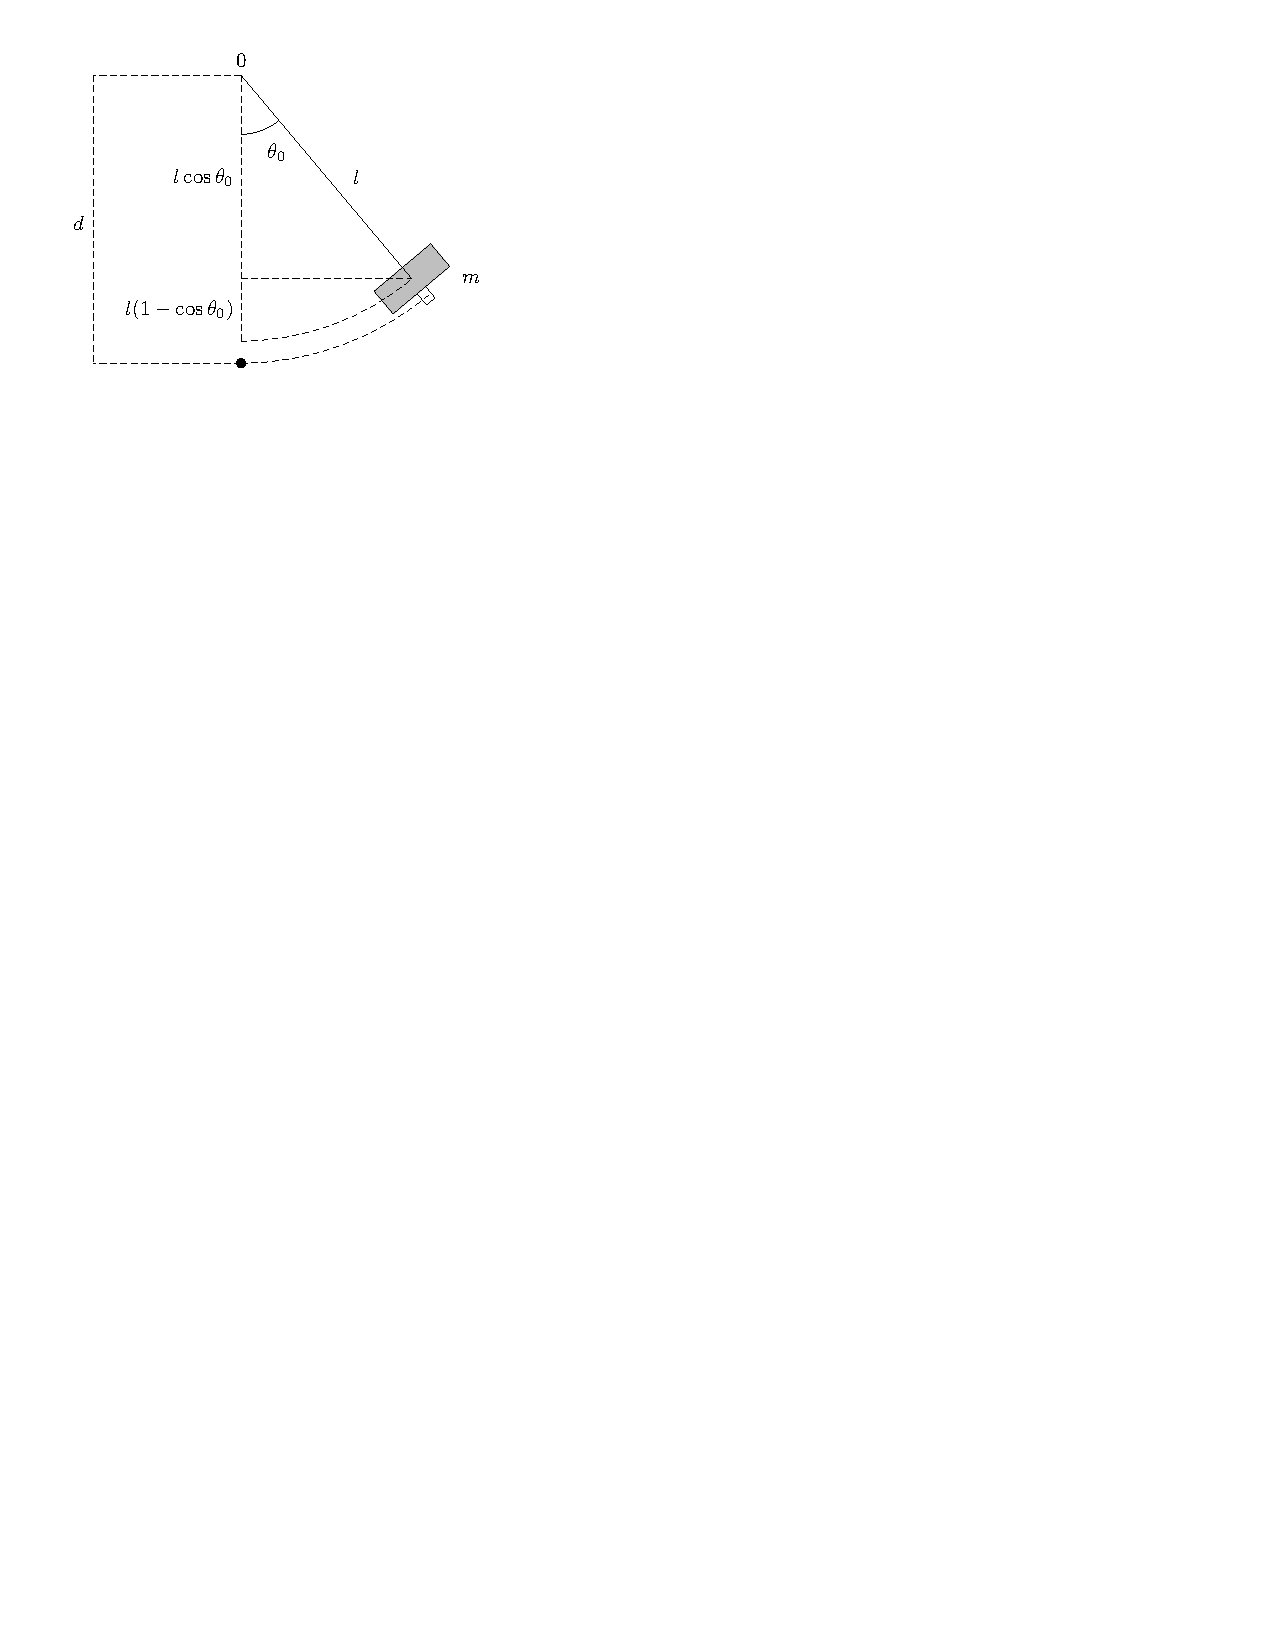
\includegraphics[scale=0.80]{pendolo_fisico_2.pdf}
  		\caption{Schematizzazione del nostro apparato sperimentale: il pendolo, nel laboratorio, è in realtà sorretto da 4 fili che agiscono, complessivamente, come un unico filo di massa trascurabile e di lunghezza $L$ che collega il perno al CM del corpo. Da notare il fatto che il punto a distanza $d$ viaggia ad una velocità maggiore, essendo ad una distanza maggiore dal perno, rispetto al centro di massa}
  		\label{fig:pendolo}
	\end{figure}	
	Per fare ciò ci siamo serviti di una fotocellula e di un programma di acquisizione che misurava ogni istante in cui il corpo attivava la fotocellula, il periodo dell'oscillazione che il pendolo stava compiendo (siccome gli attriti dell'aria non sono trascurabili) e il \emph{tempo transiente}, ovvero il tempo in cui il nostro pendolo quadrifilare andava ad oscurare con la sbarretta la fotocellula. Per effettuare ciò abbiamo misurato la lunghezza $L$, ovvero la lunghezza del CM del corpo dal perno di rotazione, la lunghezza $d$, ovvero la distanza del perno dal punto della sbarretta che verticalmente passava per la fotocellula, e la larghezza $w$ della sbarretta.
\begin{align*}
	&L = (1.150 \pm 0.001) \, \si{\meter} & &d = (1.180 \pm 0.001) \, \si{\meter} & &w = (2.050 \pm 0.005) \, \si{\centi\meter}
\end{align*}
Tramite il tempo transiente $\tau$ e la larghezza $w$ era possibile calcolare la velocità media della sbarretta nel punto a distanza $d$ quando passava per la verticale, approssimando il piccolo arco che il pendolo percorreva alla distanza $w$ misurata. Tuttavia noi eravamo interessati a calcolare la velocità del centro di massa che è possibile calcolare con la seguente formula (che si può ricavare tramite le coordinate polari e supponendo che, nell'intervallo di tempo \emph{piccolo}, rispetto alle altre grandezze in gioco, in cui passa per la fotocellula, la velocità angolare sia costante)
\begin{equation}
	v_{CM} = \frac{w}{\tau}\frac{l}{d}
\end{equation}
a cui possiamo assegnare l'incertezza tramite la seguente formula
\begin{equation}
	\sigma_{v_{CM}} = v_{CM} \sqrt{ \left( \frac{\sigma_w}{w} \right)^2 + \left( \frac{\sigma_{\tau_i}}{\tau_i} \right)^2 + \left( \frac{\sigma_l}{l} \right)^2 + \left( \frac{\sigma_d}{d} \right)^2}
\end{equation}
Tuttavia che errore possiamo assegnare a $w$? Considerando che la misura del \emph{tempo transiente} viene fatta da uno strumento digitale allora tutti i valori compresi nella sensibilità dello strumento sono equiprobabili, dunque l'errore che possiamo assegnare a $\tau_i$ è pari alla sensibilità dello strumento (pari a $4 \, \si{\micro\second}$):
$$
	\sigma_{\tau_i} = \frac{4}{\sqrt{12}} \, \si{\micro\second}
$$
Abbiamo prima effettuato il grafico del periodo in funzione del tempo, da cui ci si aspettava che il periodo $T$ diminuisse nel corso del tempo (siccome agiscono gli attriti dell'aria)
\begin{figure}[htpb]
	\centering
	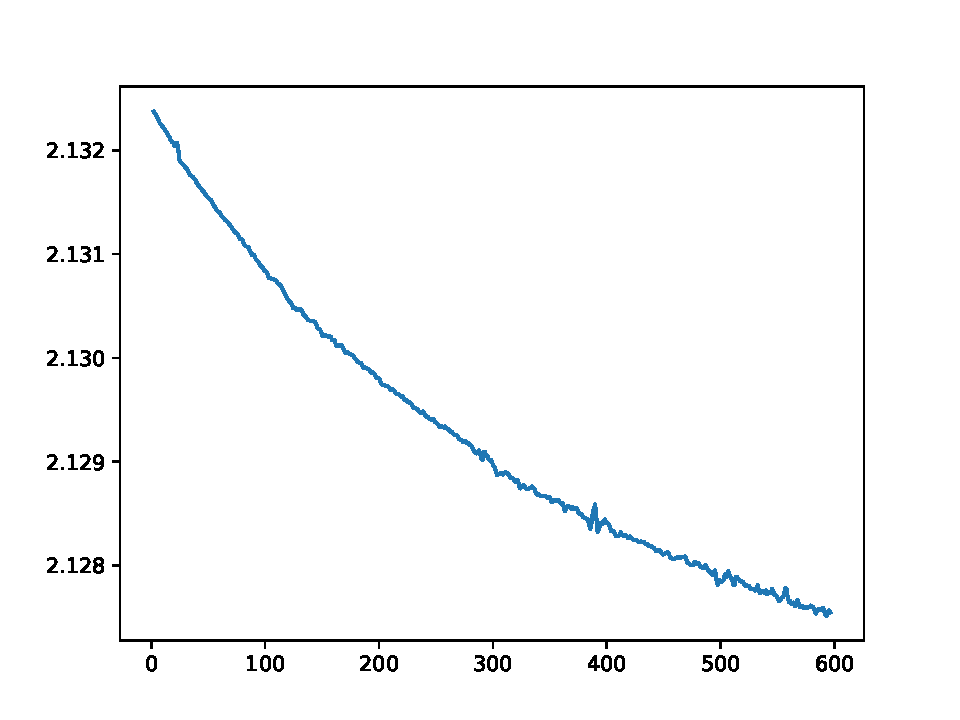
\includegraphics[scale=0.80]{Grafico_periodo_tempo.pdf}
	\caption{Grafico del periodo in funzione del tempo: si osserva che il periodo, come atteso teoricamente, diminuisce nel corso del tempo. Le \emph{spezzate} che si osservano nel grafico possono derivare da \emph{colpi} che sono stati dati inavvertitamente al banco e, siccome il pendolo era molto sensibile, si sono fatte \emph{sentire} }
\end{figure}
A quel punto, abbiamo voluto utilizzare il metodo del fit tramite parametri liberi del grafico velocità-tempo che, a causa dello smorzamento dovuto alle forze di attrito (supponendo che la forza di attrito agisca proporzionalmente alla velocità del centro di massa), deve risultare essere della forma
\begin{equation}
	v_{CM} (t) = v_{CM} (0) e^{-\lambda t}
\end{equation}
dove $v_{CM}(0)$ rappresenta la velocità posseduta dal centro di massa quando oscura la fotocellula la prima volta. Si riporta il fit utilizzando $v_{CM} (0)$ e $\lambda$ come parametri liberi qua sotto:
\begin{figure}[htbp]
	\centering
	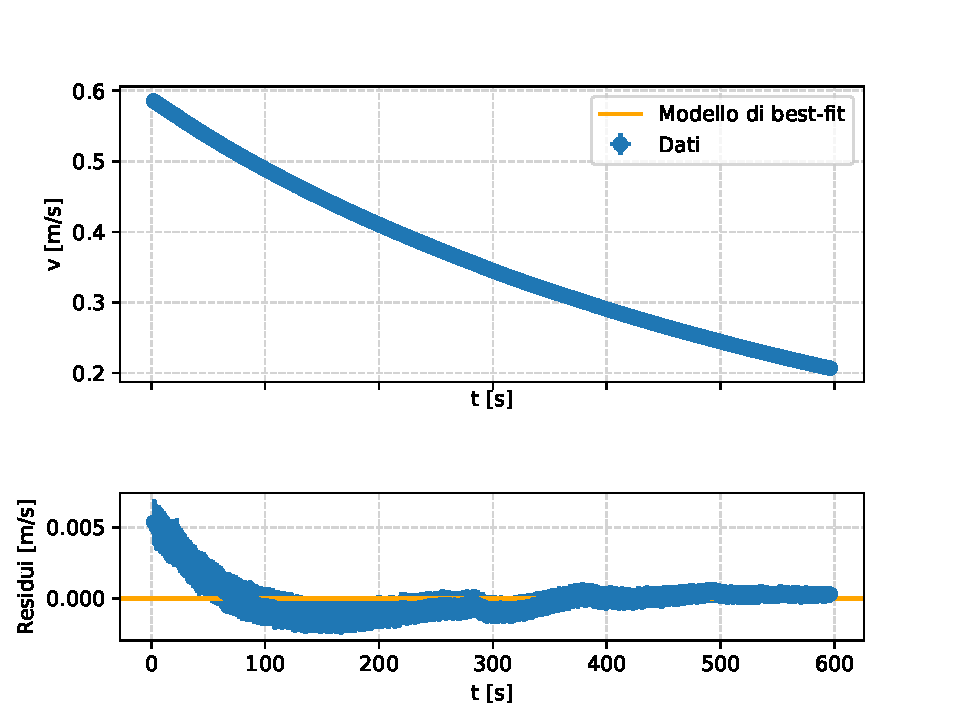
\includegraphics[scale=0.80, width=0.6\textwidth]{Fit_velocita.pdf}
	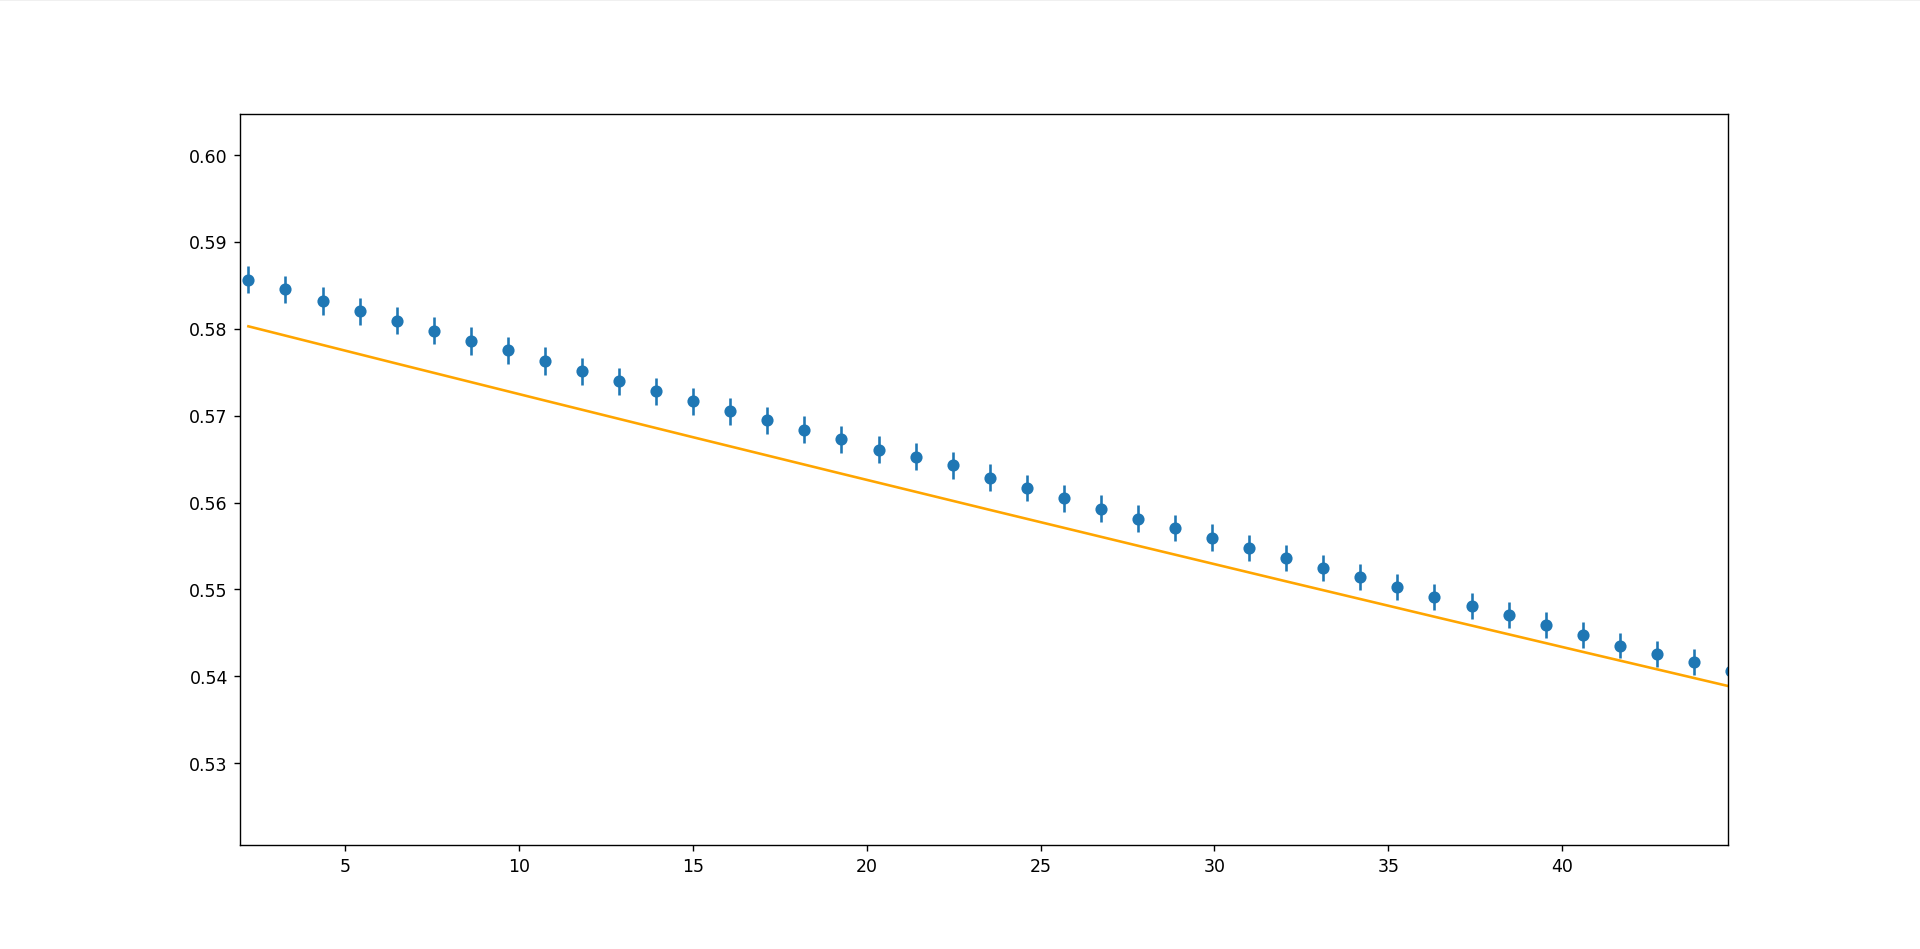
\includegraphics[scale=0.50, width=0.6\textwidth, height=6cm]{pendolo_quadrifilare_zoom.png}
	\caption{Fit del modello teorico e zoom di esso: si osserva che il fit, almeno a priori di un'analisi dei residui, risulta essere \emph{buono} siccome}
\end{figure}
Effettuando l'analisi del $\chi_2$, si osserva che, questo risulta essere circa
$$
	\chi^2 \approx 410
$$
e, in questo caso, abbiamo un numero di gradi di libertà del fit pari a $557$. Sebbene il valore del $\chi_2$ si discosta significativamente dal valore atteso, è comunque abbastanza \emph{ragionevole} siccome stiamo operando con un modello che tiene conto delle forze di attrito come proporzionali alla velocità, ma ne trascura effetti come la forma del corpo che però ne influenzano il moto. \\
\end{document}